\documentclass[12pt, a4paper, oneside]{ctexart}
\usepackage{amsmath, amsthm, amssymb, graphicx}
\usepackage{hyperref}
\usepackage{listings}
\usepackage{xcolor}
\usepackage{color}
\usepackage{enumerate}
\usepackage{epstopdf}
\usepackage{float}
\usepackage{framed}
\usepackage[ruled,vlined]{algorithm2e}
\hypersetup{
    colorlinks=true,
    linkcolor=blue,
    filecolor=blue,      
    urlcolor=blue,
    citecolor=cyan,
}
\definecolor{dkgreen}{rgb}{0,0.6,0}
\definecolor{gray}{rgb}{0.5,0.5,0.5}
\definecolor{mauve}{rgb}{0.58,0,0.82}
\definecolor{shadecolor}{rgb}{0.5,0.5,0.5}
\lstset{ %
    language=Python,                % the language of the code
    basicstyle=\footnotesize,           % the size of the fonts that are used for the code
    numbers=left,                   % where to put the line-numbers
    %numberstyle=\tiny\color{gray},  % the style that is used for the line-numbers
    %stepnumber=2,                   % the step between two line-numbers. If it's 1, each line 
                            % will be numbered
    %numbersep=5pt,                  % how far the line-numbers are from the code
    %backgroundcolor=\color{blue},      % choose the background color. You must add \usepackage{color}
    showspaces=false,               % show spaces adding particular underscores
    %showstringspaces=false,         % underline spaces within strings
    showtabs=false,                 % show tabs within strings adding particular underscores
    frame=single,                   % adds a frame around the code
    rulecolor=\color{black},        % if not set, the frame-color may be changed on line-breaks within not-black text (e.g. commens (green here))
    tabsize=2,                      % sets default tabsize to 2 spaces
    captionpos=b,                   % sets the caption-position to bottom
    breaklines=true,                % sets automatic line breaking
    breakatwhitespace=false,        % sets if automatic breaks should only happen at whitespace
    % title=\lstname,                   % show the filename of files included with \lstinputlisting;
                            % also try caption instead of title
    keywordstyle=\color{blue},          % keyword style
    commentstyle=\color{dkgreen},       % comment style
    stringstyle=\color{mauve},         % string literal style
    escapeinside={\%*}{*)},            % if you want to add LaTeX within your code
    morekeywords={*,...}               % if you want to add more keywords to the set
}
\title{ICS\_Lab4\_Report}
\author{Xiaoma}
\date{\today}
\begin{document}
\maketitle
\section*{实验目的}
使用LC-3汇编命令实现对16个人的成绩的升序排列,并求出这16个人中获得
评级A,B的数量。\\
已知当该同学的成绩为85分及以上,且其排名为25\%时,评级为A。\\
当该同学的成绩低于85分但大于等于75分,且其排名为50\%时,评级为B。
\begin{itemize}
    \item 16个人的成绩存储在以\verb|x4000|开始的连续内存空间中
    \item 每个人的成绩都在0-100之间,且每个人的成绩都不相同
    \item 排序后的成绩存储在以\verb|x5000|开始的连续内存空间中
    \item 评级A,B的数量存储在内存位置\verb|x5100|,\verb|x5101|中
\end{itemize}

\section*{实验原理}
为了降低代码复杂度,我们使用选择排序的方式,
既要对16个人的程序进行升序排列,又要统计评级A,B的数量,已知A,B既有分数限制
又有排名限制,所以如果在升序排序的同时判断评级,则会因无法判断其排名而得到正确结果。
所以我们采用降序排序的同时判断评级,最后逆序存储序列。\\
根据该思想可以得到伪代码:
\begin{algorithm*}
    \caption{mySort}
    \label{alg:algorithm}
    \KwIn{The scores of students: score[16];}
    \KwOut{The number of A: num\_a; The number of B: num\_b;}
    \BlankLine
    num\_a = 0\;
    num\_b = 0\;
    \For(){$i = 0; i < 16; ++i$}{
        max = i\;
        j = i\;
        \For(){$;j < 16; ++j$}{
            \If(){score[max] < score[j]}{
                max = j;
            }
        }
        swap(score[max], score[i])\;
        \If(){$score[i] >= 85 \& \& num\_a < 4$}{
            num\_a += 1;
        }
        \ElseIf(){$score[i] >= 85 \& \& num\_a + num\_b < 8$}{
            num\_b += 1;
        }
        \ElseIf(){$score[i] >= 75 \& \& num\_a + num\_b < 8$}{
            num\_b += 1;
        }
    }
    \Return{$num\_a,num\_b$};
\end{algorithm*}

\section*{实验步骤}
\subsection*{选择排序的实现}
对于通常情况下的选择排序,第二次循环起始位置应该为初始$max$的下一个位置,但若果这样做,会导致两个循环的判断终止条件
不同,为了降低代码复杂度,设定第二次循环的起始位置为$max$。
\subsection*{判断评级}
设定$num\_a,num\_b$为此时评级为A,B的数量。\\
$\begin{cases}
    num\_a += 1 \quad score \geq 85,num\_a < 4\\
    num\_b += 1 \quad score \geq 85,num\_a + num\_b < 8 , num\_a \geq 4 \\
    num\_b += 1 \quad 75 \leq score < 85,num\_a + num\_b < 8
\end{cases}$
\subsection*{倒序存储}
对降序排序的序列进行倒序存储,得到的即为正向的升序排列。
\subsection*{代码讲解}
\subsubsection*{初始化变量}
将$R0$作为16个成绩的指针,$R1$为循环的最后一个位置,$R6,R7$存储评级
A,B的数量,即
$$R0 \leftarrow \& score, R1 \leftarrow \& score[15]$$
\begin{lstlisting}[name = code, firstnumber = 1]
    LD R0, SCORE
    ADD R1, R0, #15
    AND R6, R6, #0
    AND R7, R7, #0
\end{lstlisting}
\subsubsection*{外部循环}
选择排序的外部循环,初始化$max,j$后进入内部循环,从内部循环返回后,进入$JUDGE$判断评级,
然后将局部最大值写入相应位置,逆序存储结果,循环结束时,进入$STORE$存储评级结果,即
$$swap(score[max], score[i])$$
$$sortScore[16-i] \leftarrow score[i]$$
\begin{lstlisting}[name = code, firstnumber = last]
    LOOPA 
    AND R2, R2, #0
    ADD R2, R0, #0
    AND R3, R3, #0
    ADD R3, R0, #0
    BRnzp LOOPB
    RETB
    LDR R4, R2, #0
    LDR R5, R0, #0
    STR R4, R0, #0
    STR R5, R2, #0
    LD R3, RESULTS
    LD R2, SCORE
    ADD R3, R2, R3
    NOT R2, R0
    ADD R2, R2, #1
    ADD R2, R2, R1
    ADD R3, R3, R2
    STR R4, R3, #0
    BRnzp JUDGE
    RETJ
    ADD R0, R0, #1
    NOT R4, R0
    ADD R4, R4, #1
    ADD R4, R1, R4
    BRn STORE
    BRnzp LOOPA
\end{lstlisting}
\subsubsection*{内部循环}
选择排序的内部循环,若当前指针指向的值大于$max$指向的值,则更新$max$,即
$$max \leftarrow argmax_{x \in \{ max, j \}  }(score[x])$$
\begin{lstlisting}[name = code, firstnumber = last]
    LOOPB
    LDR R4, R2, #0
    LDR R5, R3, #0
    NOT R4, R4
    ADD R4, R4, #1
    ADD R4, R5, R4
    BRnz #2
    AND R2, R2, #0
    ADD R2, R3, #0
    ADD R3, R3, #1
    NOT R4, R3
    ADD R4, R4, #1
    ADD R4, R1, R4
    BRzp LOOPB
    BRnzp RETB
\end{lstlisting}
\subsubsection*{判断评级}
若成绩不低于85且排名不低于25\%,则评级A;若成绩不低于85且排名低于25\%高于50\%,则评级B;
若成绩低于85不低于75且排名低于25\%高于50\%,则评级B,即
$$\begin{cases}
    num\_a += 1 \quad score \geq 85,num\_a < 4\\
    num\_b += 1 \quad score \geq 85,num\_a + num\_b < 8, num\_a \geq 4  \\
    num\_b += 1 \quad 75 \leq score < 85,num\_a + num\_b < 8
\end{cases}$$
\begin{lstlisting}[name = code, firstnumber = last]
    JUDGE
    LDR R4, R0, #0
    LD R5, SCOREMARKA 
    ADD R4, R4, R5
    BRn #4
    ADD R5, R6, #-4
    BRz #4
    ADD R6, R6, #1
    BRnzp RETJ
    ADD R4, R4, #10
    BRn RETJ
    ADD R5, R6, R7
    ADD R5, R5, #-8
    BRz RETJ
    ADD R7, R7, #1
    BRnzp RETJ
\end{lstlisting}
\subsubsection*{存储结果}
分别将评级A,B的数量存储到对应地址,即
$$mem[\verb|x5100|] \leftarrow num\_a$$
$$mem[\verb|x5101|] \leftarrow num\_b$$
\begin{lstlisting}[name = code, firstnumber = last]
    STORE
    STI R6, RESULTA
    STI R7, RESULTB
\end{lstlisting}

\section*{实验结果}
依次对实验文档给出的例子进行测试,结果如下:
\begin{figure}[H]
    \centering
    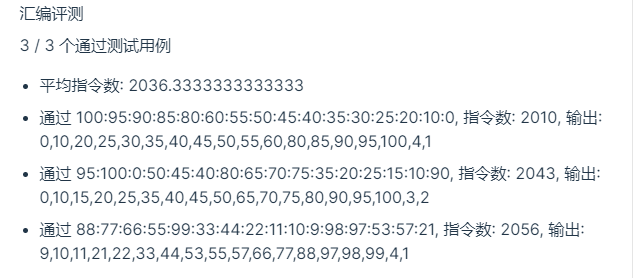
\includegraphics[scale=0.8]{Output1.png}
\end{figure}
自行编写了部分测试例子,分别考虑了评级的几种不同情况,结果如下:
\begin{figure}[H]
    \centering
    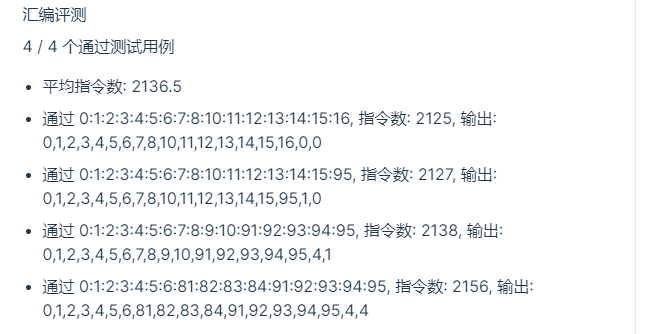
\includegraphics[scale=0.8]{Output2.png}
\end{figure}

\end{document}